\documentclass[aspectratio=169, 10pt]{beamer}

\usetheme{Madrid}
\usecolortheme{whale}

% Typography & Colors
\definecolor{NavyBlue}{RGB}{15, 32, 67}
\definecolor{SlateBlue}{RGB}{30, 58, 138}
\definecolor{AccentCyan}{RGB}{14, 165, 233}
\definecolor{EmeraldGreen}{RGB}{16, 185, 129}
\definecolor{CrimsonRed}{RGB}{225, 29, 72}
\definecolor{DarkSlate}{RGB}{30, 41, 59}
\definecolor{LightGray}{RGB}{248, 250, 252}

\setbeamercolor{palette primary}{bg=NavyBlue, fg=white}
\setbeamercolor{palette secondary}{bg=SlateBlue, fg=white}
\setbeamercolor{palette tertiary}{bg=DarkSlate, fg=white}
\setbeamercolor{structure}{fg=SlateBlue}
\setbeamercolor{titlelike}{parent=palette primary}
\setbeamercolor{block title}{bg=SlateBlue, fg=white}
\setbeamercolor{block body}{bg=LightGray, fg=DarkSlate}

\setbeamertemplate{navigation symbols}{}
\setbeamertemplate{footline}{
  \leavevmode%
  \hbox{%
  \begin{beamercolorbox}[wd=.333333\paperwidth,ht=2.25ex,dp=1ex,center]{author in head/foot}%
    \usebeamerfont{author in head/foot}Brian A. Hadian
  \end{beamercolorbox}%
  \begin{beamercolorbox}[wd=.333333\paperwidth,ht=2.25ex,dp=1ex,center]{title in head/foot}%
    \usebeamerfont{title in head/foot}Phase 0 Architecture Audit
  \end{beamercolorbox}%
  \begin{beamercolorbox}[wd=.333333\paperwidth,ht=2.25ex,dp=1ex,right]{date in head/foot}%
    \usebeamerfont{date in head/foot}\insertframenumber{} / \inserttotalframenumber\hspace*{2ex}
  \end{beamercolorbox}}%
  \vskip0pt%
}

\usepackage{graphicx}
\usepackage{booktabs}
\usepackage{amsmath}
\usepackage{amssymb}
\usepackage{tikz}
\usetikzlibrary{positioning}

\title[Phase 0 Architecture Audit]{\textbf{Phase 0 Architecture Audit: Mechanistic Discovery Framework}}
\subtitle{System Decomposition, Parameter Inventory, and Operational Boundaries}
\author{\textbf{Brian A. Hadian}}
\institute[Embedded AI \& Robotics]{\textbf{Project Hephaestus: Autonomous Robotics \& Hardware Lab}}
\date{\today}

\begin{document}

% ============================================================================
% SLIDE 1: Title Slide
% ============================================================================
\begin{frame}
  \titlepage
  \begin{center}
    \footnotesize \textcolor{SlateBlue}{\textbf{Research Mandate:}} Reverse-engineer language-grounded world models to extract causally essential circuits for FPGA acceleration.
  \end{center}
\end{frame}

% ============================================================================
% SLIDE 2: Model Inventory & Parameter Breakdown
% ============================================================================
\begin{frame}{Parameter Inventory: 100\% Accountability Across Architectures}
  \begin{columns}
    \begin{column}{0.54\textwidth}
      \begin{block}{\textbf{One Core Insight}}
        Every trainable tensor (72 parameters across 3 models) has been mapped, classified, and verified against SHA-256 checkpoint fingerprints.
      \end{block}
      \vspace{0.3em}
      \begin{itemize}
        \footnotesize
        \item \textbf{Baseline Navigation Policy}: 147,028 parameters ($z \in \mathbb{R}^{32}$, 1-step direct visual policy).
        \item \textbf{LeWorldModel (LeWM)}: 148,913 parameters (Conv4-LN encoder + action-conditioned residual transition core + SIGReg).
        \item \textbf{H-JEPA}: 166,037 parameters (Shared visual encoder + Macro Predictor at stride $K=5$ + Micro tracking policy).
      \end{itemize}
    \end{column}
    \begin{column}{0.44\textwidth}
      \centering
      \scriptsize
      \begin{tabular}{lcc}
        \toprule
        \textbf{Model} & \textbf{Parameters} & \textbf{Status} \\
        \midrule
        Baseline Policy & 147,028 & Verified \\
        LeWorldModel & 148,913 & Verified \\
        H-JEPA & 166,037 & Verified \\
        \midrule
        \textbf{Total Audited} & \textbf{461,978} & \textbf{100\% Accounted} \\
        \bottomrule
      \end{tabular}
      \vspace{0.8em}
      \begin{alertblock}{Integrity Check}
        All checkpoints SHA-256 hashed and locked in \texttt{research/audit/parameter\_inventory.csv}.
      \end{alertblock}
    \end{column}
  \end{columns}
\end{frame}

% ============================================================================
% SLIDE 3: Learned vs Engineered Boundaries
% ============================================================================
\begin{frame}{System Boundary: Separating Learned Intelligence from Heuristics}
  \begin{columns}
    \begin{column}{0.54\textwidth}
      \begin{block}{\textbf{One Core Insight}}
        Language parsing and flank routing are deterministic software, whereas visual dynamics and collision prediction are learned neural computations.
      \end{block}
      \vspace{0.3em}
      \begin{itemize}
        \footnotesize
        \item \textbf{Deterministic NLP Layer}: Regex keyword matching and spatial geometry calculate target poses and clearance flanks with zero neural weights.
        \item \textbf{Learned Neural Layer}: 4-layer CNN feature extraction, latent transition foresight ($\Delta s$), and collision probability prediction.
        \item \textbf{Discovery Implication}: Mechanistic discovery must evaluate latent foresight directly without confounding it with engineered waypoints.
      \end{itemize}
    \end{column}
    \begin{column}{0.44\textwidth}
      \centering
      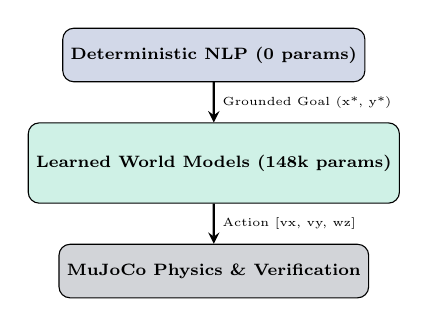
\begin{tikzpicture}[scale=0.85, every node/.style={transform shape}]
        \node[draw, fill=SlateBlue!20, rounded corners, minimum width=4cm, minimum height=0.8cm, font=\scriptsize\bfseries] (nlp) {Deterministic NLP (0 params)};
        \node[draw, fill=EmeraldGreen!20, rounded corners, minimum width=4cm, minimum height=1.2cm, font=\scriptsize\bfseries, below=0.6cm of nlp] (nn) {Learned World Models (148k params)};
        \node[draw, fill=DarkSlate!20, rounded corners, minimum width=4cm, minimum height=0.8cm, font=\scriptsize\bfseries, below=0.6cm of nn] (sim) {MuJoCo Physics \& Verification};
        \draw[->, thick, >=stealth] (nlp) -- node[right, font=\tiny] {Grounded Goal (x*, y*)} (nn);
        \draw[->, thick, >=stealth] (nn) -- node[right, font=\tiny] {Action [vx, vy, wz]} (sim);
      \end{tikzpicture}
    \end{column}
  \end{columns}
\end{frame}

% ============================================================================
% SLIDE 4: Operational Graph & FPGA Acceleration Boundary
% ============================================================================
\begin{frame}{Operational Graph: Locating the FPGA Acceleration Boundary}
  \begin{columns}
    \begin{column}{0.52\textwidth}
      \begin{block}{\textbf{One Core Insight}}
        The $0.48\,\mu\text{s}$ FPGA measurement isolates the MLP predictor core; end-to-end inference includes observation capture and CNN encoding.
      \end{block}
      \vspace{0.3em}
      \begin{itemize}
        \footnotesize
        \item \textbf{PL Accelerated Core}: 3-layer MLP transition/policy network (6,788 - 8,609 MACs) running at 48 clock cycles ($0.48\,\mu\text{s}$ @ 100~MHz).
        \item \textbf{PS Host Tasks}: Camera rendering ($2.1\,\text{ms}$) and CNN visual encoding ($4.8\,\text{ms}$ on ARM / $0.06\,\text{ms}$ on GPU).
        \item \textbf{Circuit Extraction Target}: Phase 7 will investigate whether the visual encoder itself can be pruned into a compact circuit deployed to PL.
      \end{itemize}
    \end{column}
    \begin{column}{0.46\textwidth}
      \centering
      \resizebox{\columnwidth}{!}{%
      \begin{tabular}{lcc}
        \toprule
        \textbf{Operation} & \textbf{Hardware Domain} & \textbf{Latency} \\
        \midrule
        Camera Frame Capture & Host MuJoCo & $\approx 2.1\,\text{ms}$ \\
        Visual CNN Encoder & Host CPU / GPU & $4.8\,\text{ms}$ / $60\,\mu\text{s}$ \\
        AXI-Lite PS-PL Write & AXI4-Lite Bus & $0.72\,\mu\text{s}$ \\
        \textbf{Predictor PL Kernel} & \textbf{KR260 FPGA PL} & \textbf{0.48 $\mu$s} \\
        AXI-Lite PL-PS Read & AXI4-Lite Bus & $0.64\,\mu\text{s}$ \\
        Control Timestep & Host AMR Loop & $100\,\text{ms}$ (10 Hz) \\
        \bottomrule
      \end{tabular}%
      }
    \end{column}
  \end{columns}
\end{frame}

% ============================================================================
% SLIDE 5: Literature Gap Analysis
% ============================================================================
\begin{frame}{Literature Gap Analysis: Aligning Implementation with Theory}
  \begin{columns}
    \begin{column}{0.54\textwidth}
      \begin{block}{\textbf{One Core Insight}}
        Architectural downscaling to 148k parameters was essential for on-chip FPGA synthesis while preserving core JEPA and SIGReg principles.
      \end{block}
      \vspace{0.3em}
      \begin{itemize}
        \footnotesize
        \item \textbf{LeWM (arXiv:2603.19312)}: Original 15M-param ViT exceeds Kria XCK26 on-chip BRAM (1.2 MB). Compact Conv4-LN faithfully preserves SIGReg moment matching and non-generative dynamics.
        \item \textbf{H-JEPA (arXiv:2610.06805)}: 2-tier implementation ($K=5$ macro stride) matches physical JetAuto Mecanum dynamics ($0.30\,\text{m}$ clearance radius per macro step).
        \item \textbf{Methodology Verified}: Documented transparently in \texttt{research/audit/implementation\_deviations.md}.
      \end{itemize}
    \end{column}
    \begin{column}{0.44\textwidth}
      \centering
      \begin{block}{Theoretical Alignment}
        \tiny
        \textbf{LeWM SIGReg Objective:}
        $$\mathcal{L} = \frac{1}{B}\sum \|\hat{s}_{t+1} - \text{sg}(s_{t+1})\|^2 + \lambda_{\text{reg}}\mathcal{L}_{\text{SIGReg}}(s)$$
        \textbf{H-JEPA Hierarchy:}
        $$\text{Macro: } \hat{S}_{k+1} = T_{\text{macro}}(S_k, A^{\text{macro}}_k)$$
        $$\text{Micro: } a_t = \pi_{\text{micro}}(s_t, \hat{S}_{k+1})$$
      \end{block}
    \end{column}
  \end{columns}
\end{frame}

% ============================================================================
% SLIDE 6: Verification & Prerequisites for Phase 1
% ============================================================================
\begin{frame}{Phase 0 Acceptance Verification \& Readiness for Phase 1}
  \begin{columns}
    \begin{column}{0.54\textwidth}
      \begin{block}{\textbf{One Core Insight}}
        All five Phase 0 acceptance criteria are satisfied; the foundation is established for controlled dataset generation and neural instrumentation.
      \end{block}
      \vspace{0.3em}
      \begin{itemize}
        \footnotesize
        \item \textbf{Criterion 1}: Every trainable parameter accounted for $\to$ \textbf{PASS}
        \item \textbf{Criterion 2}: Inputs/outputs identified down to shapes $\to$ \textbf{PASS}
        \item \textbf{Criterion 3}: Inference pathways fully traced $\to$ \textbf{PASS}
        \item \textbf{Criterion 4}: Checkpoints bit-exact reproducible $\to$ \textbf{PASS}
        \item \textbf{Criterion 5}: Implementation deviations documented $\to$ \textbf{PASS}
      \end{itemize}
    \end{column}
    \begin{column}{0.44\textwidth}
      \begin{alertblock}{Next Phase Prerequisites (Phase 1)}
        \footnotesize
        \begin{enumerate}
          \item Generate controlled counterfactual dataset (colors, positions, orientations).
          \item Formalize 6 capability categories.
          \item Isolate clean vs. corrupted pairs for causal activation patching.
        \end{enumerate}
      \end{alertblock}
    \end{column}
  \end{columns}
\end{frame}

\end{document}
